\documentclass[12pt,a4paper]{report}


\usepackage[utf8]{inputenc}
\usepackage{amsmath, amssymb}
\usepackage{graphicx}
\usepackage{hyperref}
\usepackage{geometry}
\geometry{margin=1in}

\hypersetup{
    colorlinks=true,
    linkcolor=blue,
    urlcolor=cyan,
    citecolor=red
}

\usepackage{titlesec}

\titleformat{\chapter}
  {\normalfont\Large\bfseries} % format
  {Problem \thechapter:}       % prints "Problem n"
  {10pt}                      % spacing between number and title
  {\Large}                     % format for the title
  [\vspace{1ex}]              % optional vertical space after

\title{\textbf{Assignment 3}\\Lagrange Interpolation Function}
\author{Sahil Raj\\\textit{2301CS41}}
\date{31 August 2025}

\begin{document}

\maketitle
\tableofcontents
\clearpage

\chapter{Interpolation of Function with Several Orders of Lagrange Interpolation Function}
\section*{Problem Statement}
The objective of this problem is to interpolate the trajectory of a projectile from observed vertical displacement data points using Newton’s Divided Difference method. From the interpolated polynomial, the goal is to estimate the projectile’s initial velocity and evaluate the accuracy of interpolation by comparing it with the actual trajectory.

\begin{quote}
  \textbf{NOTE}: The code can be accessed using this link: \href{https://raw.githubusercontent.com/HavokSahil/computational-techniques-assignments/refs/heads/main/assignment4/a1.m}{MATLAB}, \href{https://raw.githubusercontent.com/HavokSahil/computational-techniques-assignments/refs/heads/main/assignment4/a1.jl}{Julia}.
\end{quote}


\section*{Methodology}
The vertical displacement of a projectile is governed by:
\[
y(t) = v_0 t - \tfrac{1}{2} g t^2,
\]
where $v_0$ is the initial velocity and $g$ is the acceleration due to gravity. Given a discrete set of observed data points $(t_i, y_i)$, we construct an interpolating polynomial using Newton’s Divided Difference method.

\subsection*{Newton’s Divided Difference Interpolation}
1. Construct the divided difference table $D$ where:
\[
D[i,1] = y_i, \quad D[i,j] = \frac{D[i,j-1] - D[i-1,j-1]}{t_i - t_{i-j+1}}
\]
for $j \geq 2$.
2. The interpolating polynomial is:
\[
P(x) = \sum_{k=1}^N \left( D[k,k] \prod_{j=1}^{k-1}(x - t_j) \right).
\]
3. Evaluate $P(x)$ over a fine grid to approximate the trajectory.

\subsection*{Steps}
\begin{enumerate}
  \item Given time points $T = \{0,1,2,3,4\}$ and corresponding displacements $Y = \{0, 12, 18, 16, 0\}$.
  \item Construct the divided difference coefficients.
  \item Interpolate the trajectory at 10 ms resolution.
  \item Compare with the actual trajectory $y(t) = 15t - 3t^2$.
  \item Compute absolute error function $|y_{\text{interp}}(t) - y_{\text{actual}}(t)|$.
  \item Estimate the height at $t=2.5$ s.
  \item Approximate initial velocity as:
  \[
  v_0 \approx \frac{y_{\text{interp}}(t_1) - y_{\text{interp}}(t_0)}{\Delta t}.
  \]
\end{enumerate}

\section*{Results}
\begin{itemize}
  \item The interpolated polynomial closely follows the true trajectory of the projectile.
  \item The absolute error function shows minimal deviation, verifying the accuracy of interpolation.
  \item At $t=2.5$ s, the interpolated displacement was found to be:
  \[
  y(2.5) \approx \texttt{18.281250}
  \]
  \item The initial velocity was computed as:
  \[
  v_0 \approx \texttt{15.295067}
  \]
\end{itemize}

\begin{figure}[h!]
  \centering
  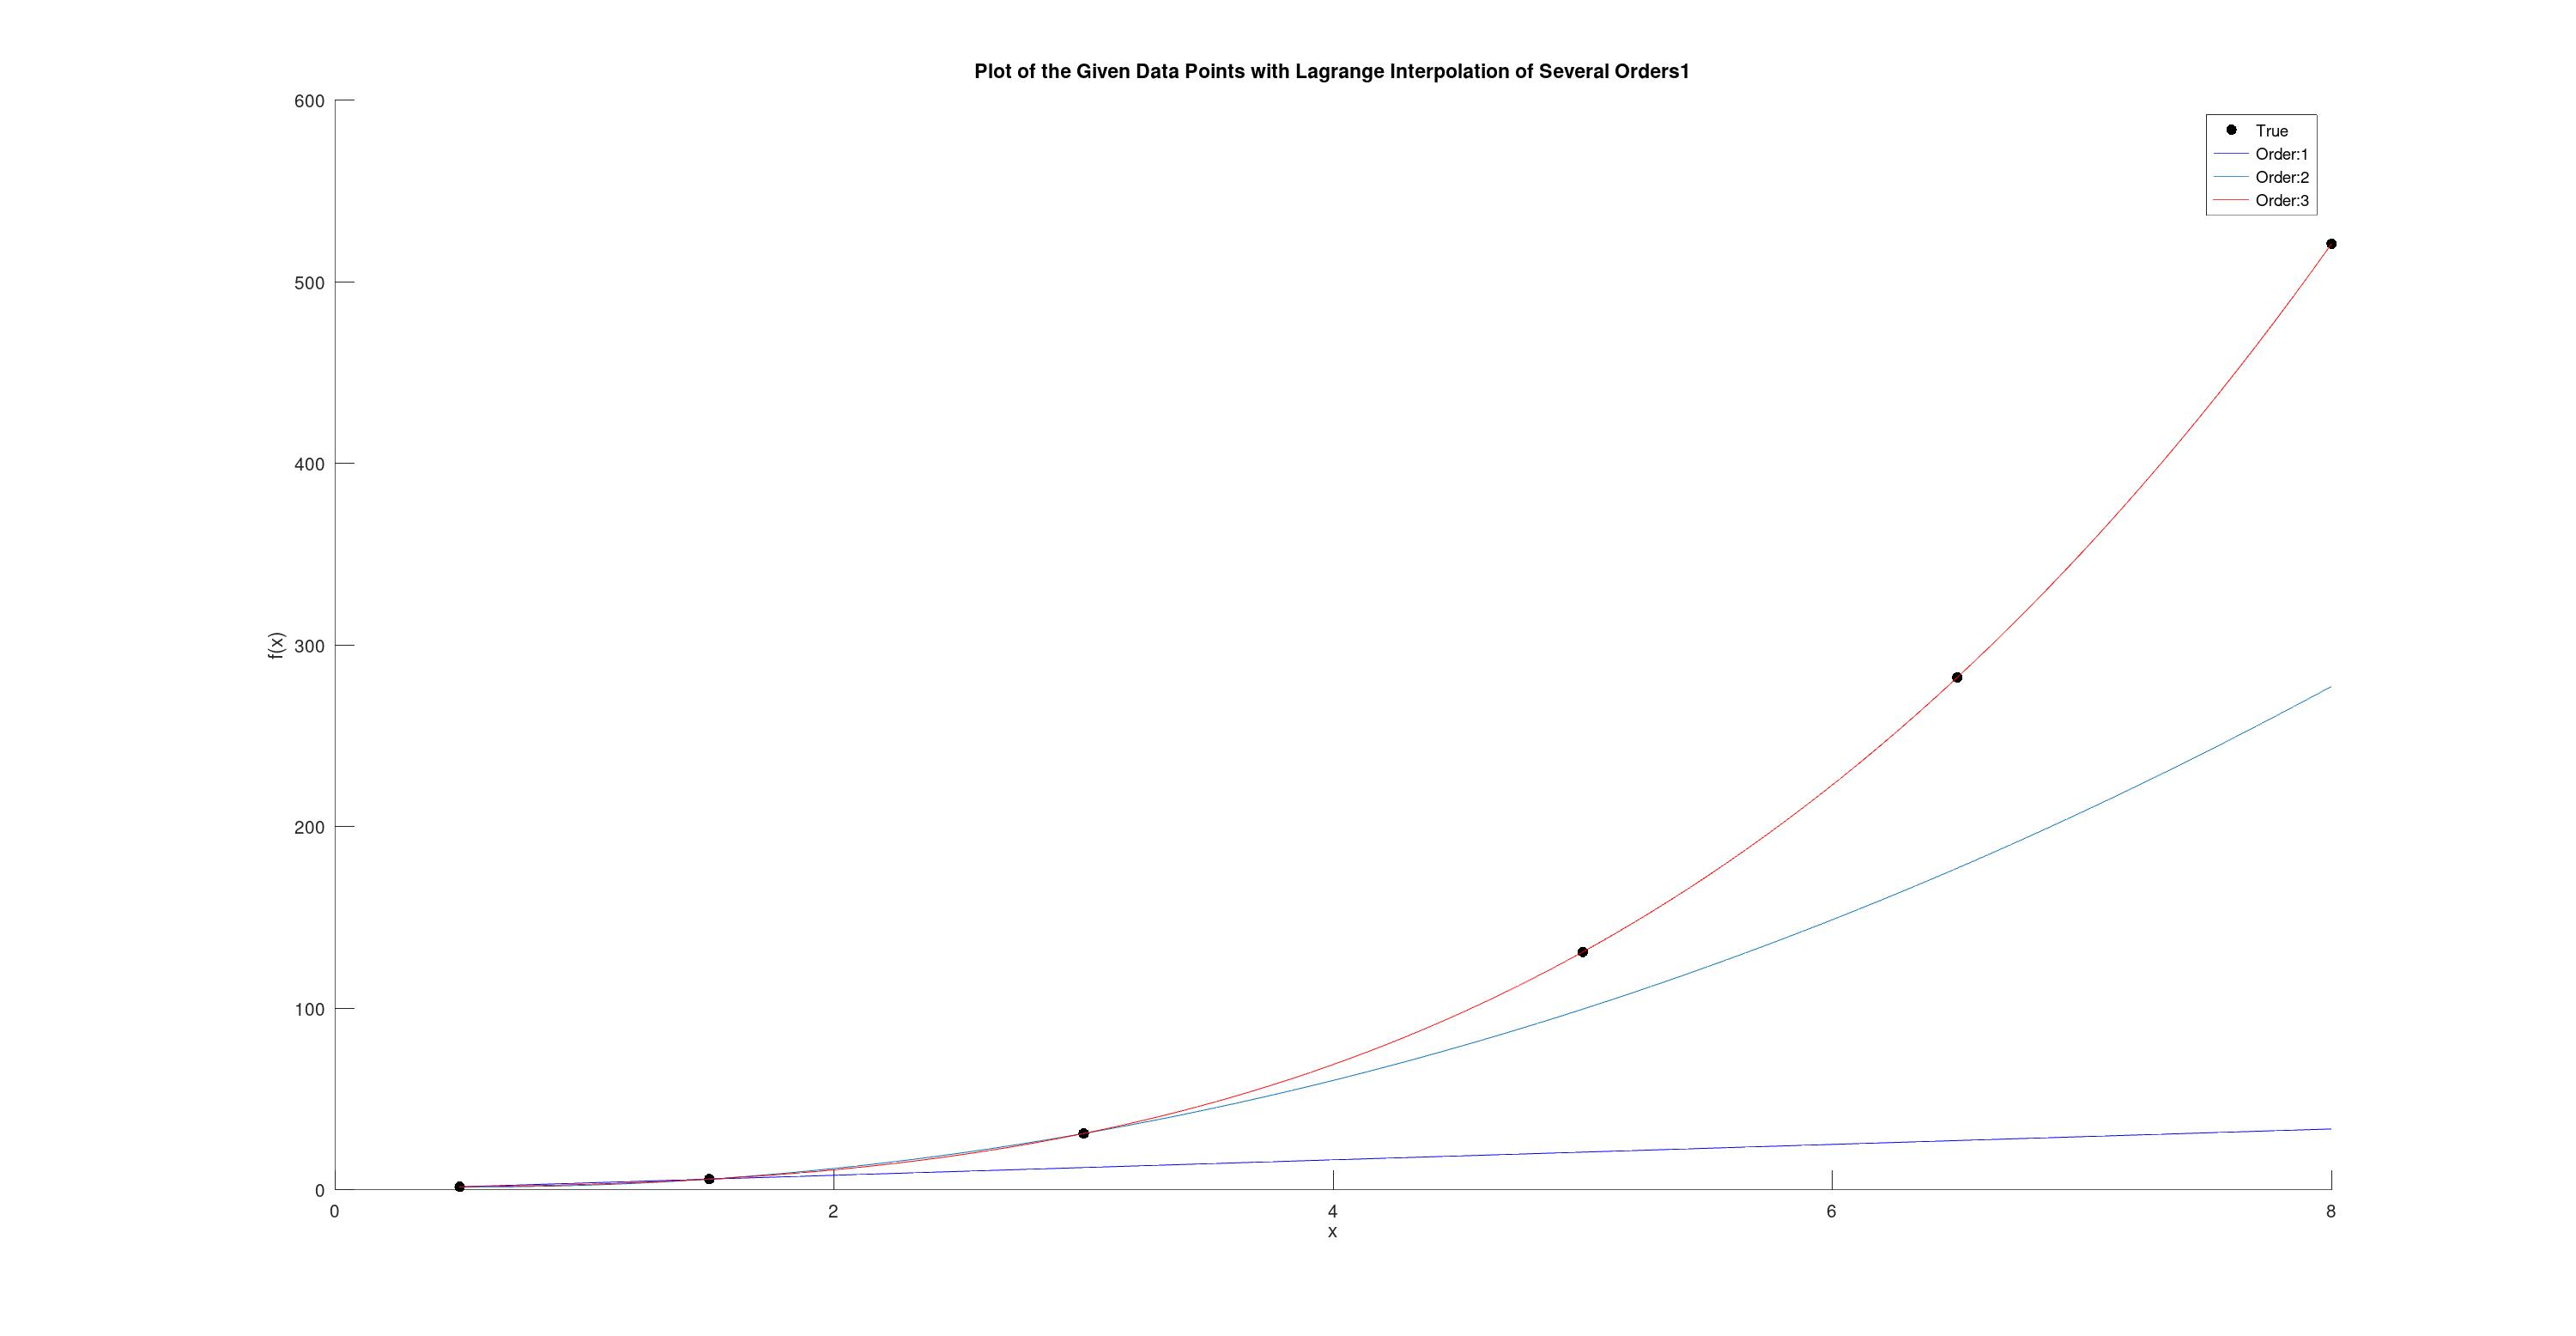
\includegraphics[width=0.93\textwidth]{a1.jpg}
  \caption{Interpolated and actual projectile trajectories (top) and absolute error function (bottom).}
\end{figure}

\section*{Conclusion}
Newton’s Divided Difference interpolation successfully reconstructed the trajectory from discrete measurements. The interpolated curve aligned closely with the analytical solution, and the estimated initial velocity was consistent with the true physical parameters. This validates polynomial interpolation as a reliable technique for analyzing projectile motion when only sparse observational data is available.


\chapter{Interpolation of Position Data of Earth around Sun}
\section*{Problem Statement} 
The objective of this problem is to solve a system of linear equations using the Gaussian elimination method with partial pivoting. Partial pivoting improves numerical stability by reducing round-off errors, especially when pivot elements are small or zero.

\section*{Methodology} 
Gaussian elimination with partial pivoting proceeds in two phases:

\begin{enumerate}
  \item \textbf{Pivoting:} At each step, reorder the rows such that the largest (by absolute value) candidate for the pivot element is placed on the diagonal. This avoids division by small numbers.
  \item \textbf{Forward elimination:} Use the pivot row to eliminate entries below the pivot, reducing the system to an upper-triangular form.
  \item \textbf{Back-substitution:} Solve for the variables starting from the last equation upwards:
  \[
  x_i = \frac{A_{i,n+1} - \sum_{j=i+1}^{n} A_{i,j}x_j}{A_{i,i}}.
  \]
\end{enumerate}

\subsection*{Pseudo-code}
\begin{enumerate}
  \item Store $M$ and $R$.
  \item Form augmented matrix $A = [M|R]$.
  \item For each pivot index $p = 1 \to n-1$:
  \begin{itemize}
    \item Swap rows to place the largest pivot in row $p$ (partial pivoting).
    \item For each row $r > p$, eliminate $A(r,p)$ using the pivot row.
  \end{itemize}
  \item Apply back-substitution to compute the solution vector.
\end{enumerate}

\section*{Results} 
The given system of equations is:
\[
\begin{aligned}
0x + 2y + z &= -8, \\
x - 2y - 2z &= 0, \\
- x + y + 2z &= 3.
\end{aligned}
\]

The augmented matrix is:
\[
A =
\begin{bmatrix}
0 & 2 & 1 & | & -8 \\
1 & -2 & -2 & | & 0 \\
-1 & 1 & 2 & | & 3
\end{bmatrix}.
\]

After applying partial pivoting, the sorted augmented matrix becomes:
\[
A =
\begin{bmatrix}
1 & -2 & -2 & | & 0 \\
0 & 2 & 1 & | & -8 \\
-1 & 1 & 2 & | & 3
\end{bmatrix}.
\]

Forward elimination reduces this system to upper-triangular form, and back-substitution yields:
\[
x = -10.00, \quad y = -3.00, \quad z = -2.00.
\]

\section*{Conclusion} 
Gaussian elimination with partial pivoting was successfully implemented to solve the given system of equations. The pivoting step ensured stability by preventing division by zero (since the original first pivot was zero). The computed solution confirms that partial pivoting is an essential enhancement to the standard Gaussian elimination method when working with arbitrary systems.



\chapter{Error Function for Interpolation of $e^{x}$ from Values at Given Points}
\section*{Problem Statement}
The objective of this problem is to compute the numerical derivative of the function \(f(x) = \cot(x)\) using \textbf{Forward Difference} and \textbf{Central Difference} schemes. The numerical derivatives are then compared with the exact analytical derivative to evaluate the accuracy of these finite difference methods.

\begin{quote}
  \textbf{NOTE}: The code can be accessed using this link: \href{https://raw.githubusercontent.com/HavokSahil/computational-techniques-assignments/refs/heads/main/assignment5/a3.m}{MATLAB}, \href{https://raw.githubusercontent.com/HavokSahil/computational-techniques-assignments/refs/heads/main/assignment5/a3.jl}{Julia}.
\end{quote}

\section*{Methodology}
The function \(f(x) = \cot(x)\) is sampled at discrete angles:
\[
X = \{1^\circ, 2^\circ, 3^\circ, 4^\circ, 5^\circ\}.
\]
These values are converted to radians for computation since MATLAB trigonometric functions use radian input.

\subsection*{Numerical Derivative Schemes}
1. \textbf{Forward Difference (FD):}
   \[
   f'(x_i) \approx \frac{f(x_{i+1}) - f(x_i)}{x_{i+1} - x_i}, \quad i = 1, \dots, N-1
   \]

2. \textbf{Central Difference (CD):}
   \[
   f'(x_i) \approx \frac{f(x_{i+1}) - f(x_{i-1})}{x_{i+1} - x_{i-1}}, \quad i = 2, \dots, N-1
   \]

3. \textbf{Exact Derivative:}
   \[
   f'(x) = -\csc^2(x)
   \]

\subsection*{Steps}
\begin{enumerate}
    \item Sample the function at the specified angles.
    \item Compute the forward difference derivative for all consecutive points.
    \item Compute the central difference derivative for interior points.
    \item Compute the exact derivative using \(-\csc^2(x)\).
    \item Plot the original function and the numerical derivatives alongside the true derivative for visual comparison.
\end{enumerate}

\section*{Results}
- The cotangent function decreases rapidly over the sampled interval.
- Forward difference derivative approximates the slope at the start of each interval, but shows slightly larger errors compared to the central difference.
- Central difference derivative provides a more accurate approximation as it uses information from both sides of a point.
- Comparison with the exact derivative shows that the central difference is closer to the true derivative across the interval.

\begin{figure}[h!]
  \centering
  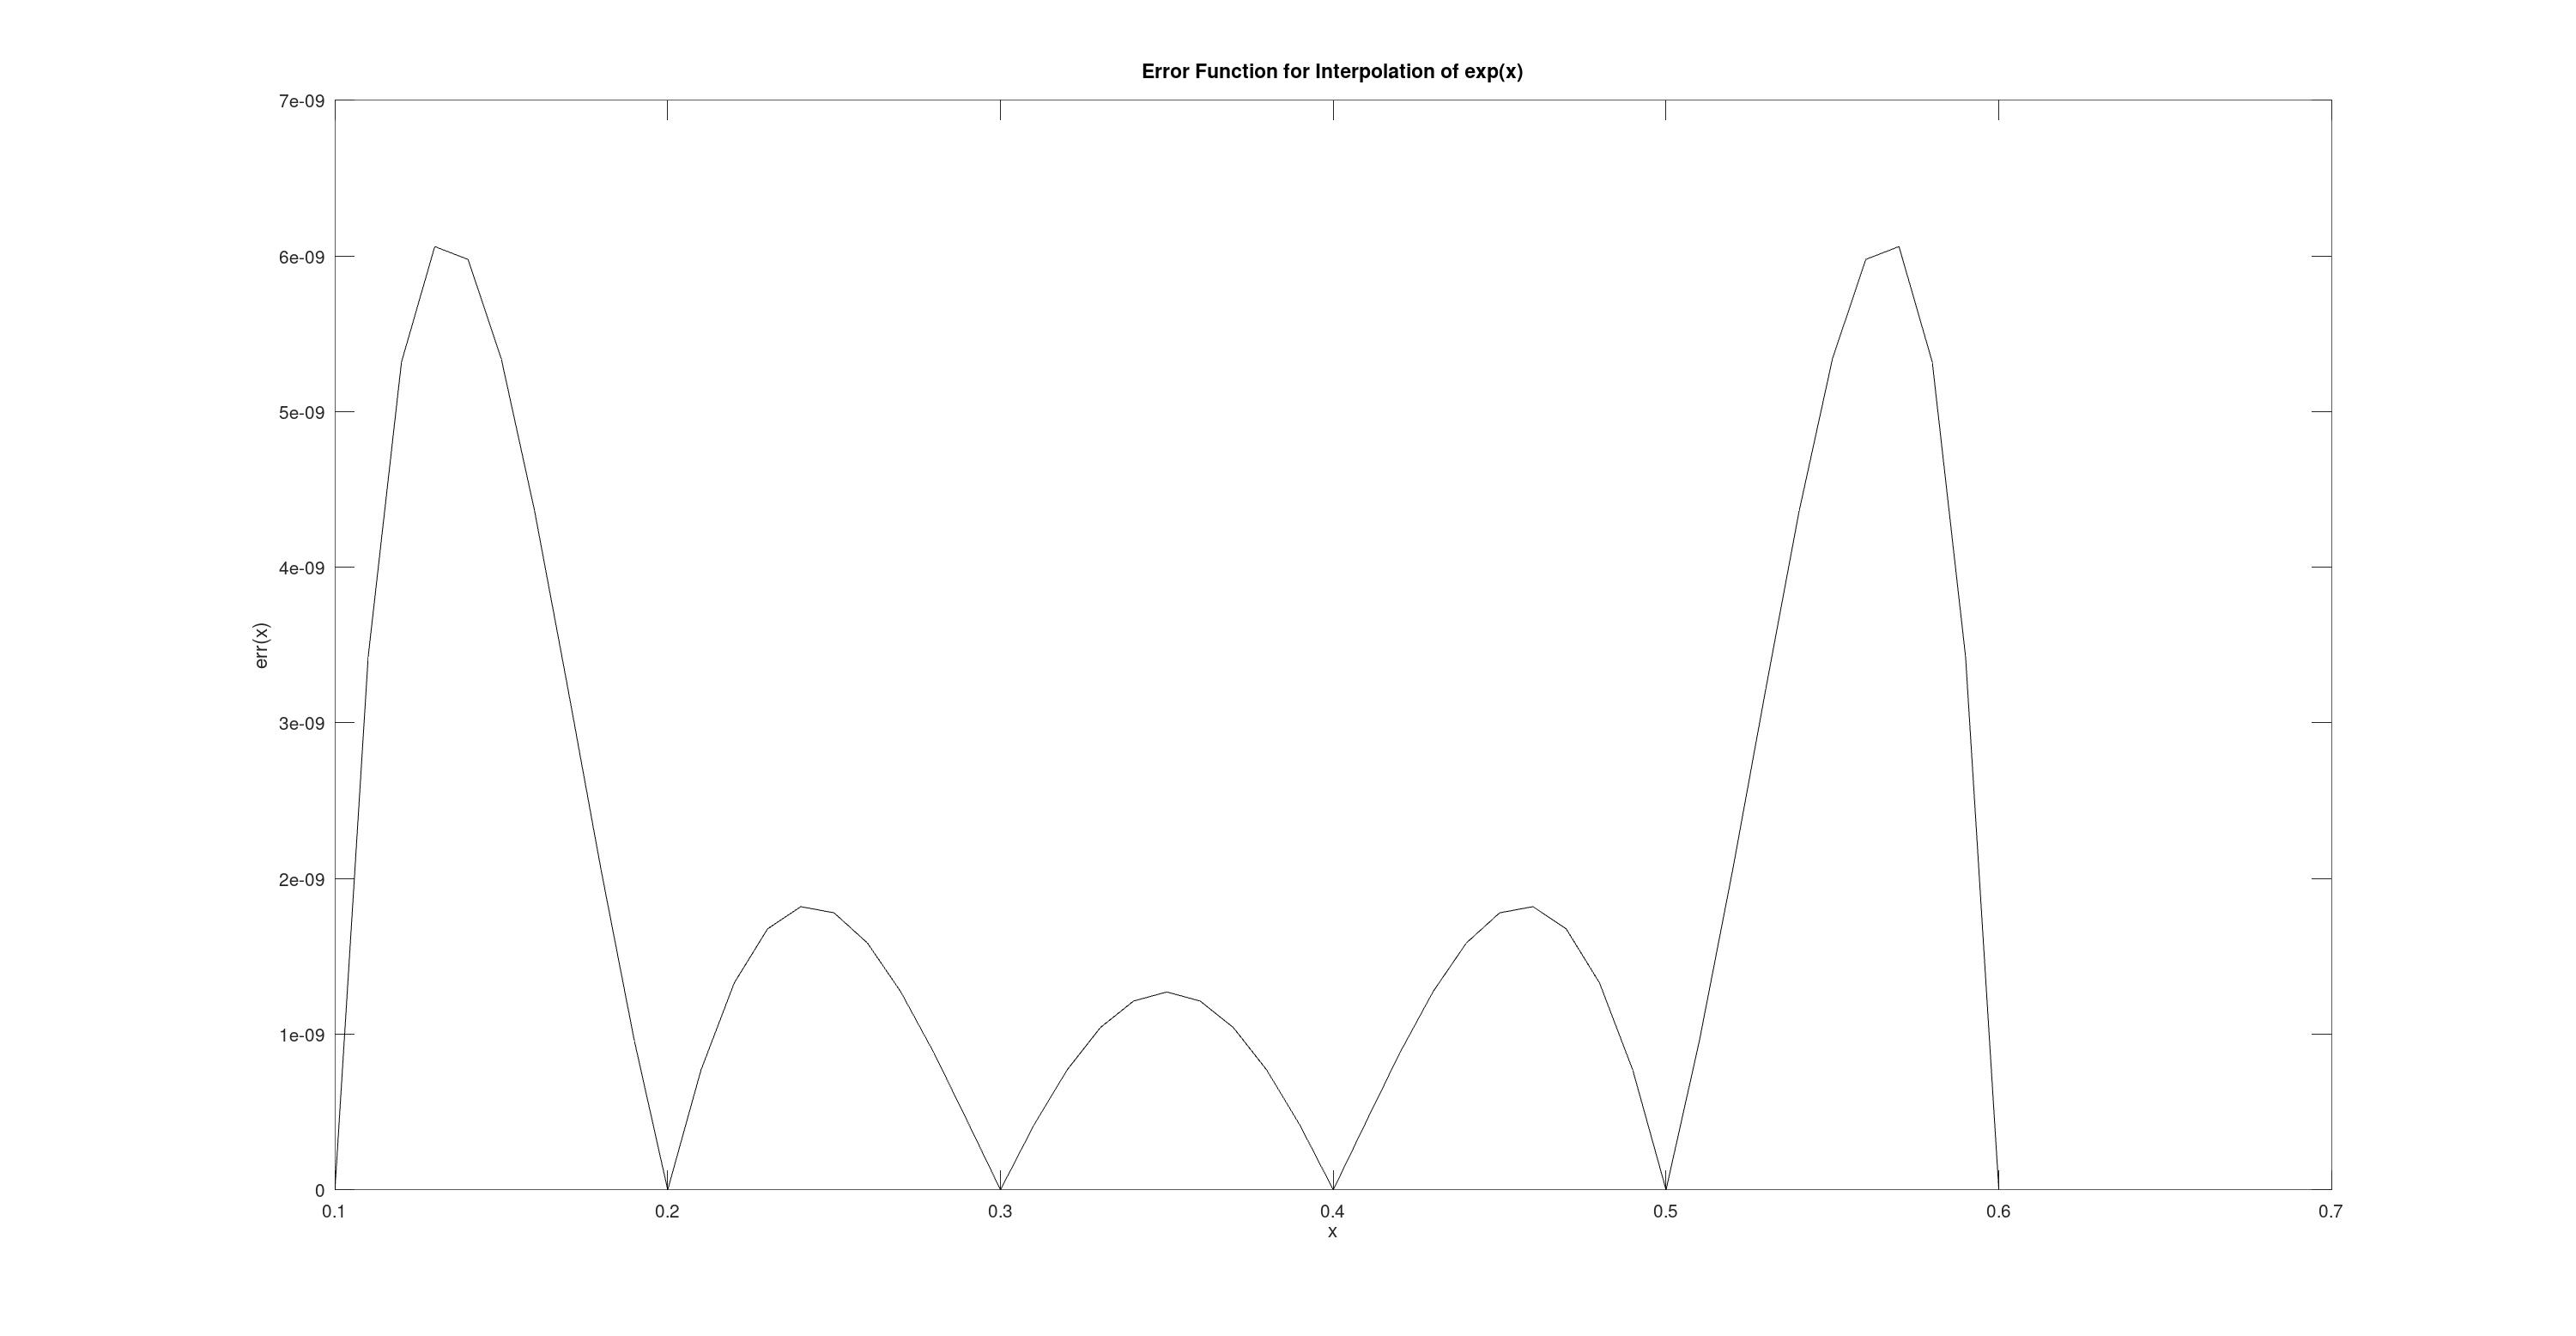
\includegraphics[width=0.9\textwidth]{a3.jpg}
  \caption{(Left) Cotangent function. (Right) Numerical derivatives using forward (red) and central (green) difference compared with the exact derivative (black dashed).}
\end{figure}

\section*{Conclusion}
Numerical differentiation using finite difference schemes successfully approximates the derivative of \(f(x) = \cot(x)\). Central difference is more accurate than forward difference due to its symmetric nature. The results validate that finite difference methods are effective for estimating derivatives of smooth functions when only discrete samples are available.


\end{document}
